The headline result of this paper is that nothing was learned about $\varphi_c$ and $\psi$.
The first result obtained, however, was that \emph{something appeared to be learned} --- and the road from the first to the second is where most of the experimental effort was spent.
We narrate it explicitly, because two genuine optimization pathologies had to be discovered, mechanistically understood, and fixed before flat loss curves could be read as evidence about physics rather than as engineering failure; and because the record of misreadings corrected along the way is the strongest argument that the final reading is not itself one of them.

\subsection{Round 1: apparent success, actual collapse}
\label{sec:phicpsi:round1}

The first full campaign (seven configurations across the five trunks) produced a beguiling number: validation $R^2 = 0.754$ for $\psi$ in the poc-mode model.
It was an artifact.
Every $\varphi_c$ prediction across the TCN variants had collapsed to a single constant (\ang{315}; $\psi$ collapsed to \ang{67.5}), with circular resultant $r_{\mathrm{circ}} = 1.000$.
For a \emph{periodic} target with uniform truth and constant prediction, the expected ``$R^2$'' computed on wrapped residuals is not 0 but exactly
\begin{equation}
    R^2_{\mathrm{null}} = 1 - \frac{\pi^2/48}{\pi^2/12} = 0.75,
\end{equation}
so 0.754 was the signature of total mode collapse, not of learning.
Meanwhile the same models' chirp-mass heads reached $R^2 > 0.95$ --- the trunk was healthy; the periodic heads specifically were dead.
This was the first of several instances in which an aggregate metric, read naively, pointed in exactly the wrong direction, and it set the tone for everything that followed: \emph{no metric was thereafter trusted until the mechanism producing it was inspected.}

\subsection{The diagnostic suite}
\label{sec:phicpsi:suite}

Seven mechanism-level checks were built incrementally during the bug hunt and re-run against every subsequent campaign: (1) true-label distribution audit; (2) loss-wiring verification; (3) uncertainty-weight and loss trajectories; (4) gradient routing --- do the periodic head weights actually change after a training step; (5) output-saturation dump; (6) end-to-end gradient-chain trace through normalization, complex multiplication, curriculum weighting, and uncertainty scaling; (7) initialization-time saturation timing.

Check~1 immediately ruled out the data pipeline: true $\varphi_c/\psi/\iota$ are uniform to $r_{\mathrm{circ}} \le 0.013$ with no duplicated or quantized values (Fig.~\ref{fig:phicpsi:labels}).
Check~2 caught a real but benign wiring fault (stale Huber-loss registrations for $\varphi_c/\psi$ alongside the poc-mode combo losses --- never invoked, but removed).
Check~4 then produced the first smoking gun: after one optimizer step, every head's predictions moved \emph{except} $\varphi_c$ and $\psi$ (mean absolute prediction change 0.15--0.81 for scalar heads, \textbf{0.00} for both angles), while --- the crucial control --- the inclination head, which shares the trunk, the two-vector encoding, and the head architecture, moved healthily.
Whatever was killing $\varphi_c/\psi$ was in their final layer, not in the trunk or the data.

\begin{figure}[tbp]
    \centering
    \includegraphics[width=\textwidth]{true_label_distributions.png}
    \caption[True label distributions]{True label distributions after HDF5
    load, before target transforms, for training (top, $n = 25{,}000$) and
    validation (bottom, $n = 5{,}000$). $\varphi_c$, $\psi$, $\iota$, and
    right ascension are uniform over their supports (circular resultant
        $\le 0.013$); declination follows the non-uniform sky prior. The
        prediction collapse observed in training is not a data-pipeline
        artifact.}
    \label{fig:phicpsi:labels}
\end{figure}

\subsection{Pathology I: output saturation at initialization}
\label{sec:phicpsi:pathology1}

Check~6's forward-pass dump found the mechanism.
Every sample's raw $\varphi_c$ output was exactly $(-1.000000, +1.000000)$ --- norm $\sqrt{2} = 1.4142$ --- and had been from \textbf{step~0}: the periodic heads used a $\tanh$ output activation, and at random initialization the pre-activation logits were already large enough to saturate it.
At saturation $\tanh' \approx 0$, so although the gradient flowing \emph{into} the output was healthy ($\lVert \partial\mathcal{L}/\partial \mathbf{z}_{\mathrm{raw}} \rVert \approx 0.31$), the gradient reaching the weights was numerically zero (kernel gradient 0.000000; bias $3.7 \times 10^{-10}$).
Adam's momentum still moved the weights (kernel change of 2.46 after a step) without ever changing the predictions --- the model was, in the record's phrase, \emph{born dead}.
The constant $\sqrt{2}$ also retro-explained the frozen std\_ratio $= 1.4142$ seen in every earlier trajectory.

The fix is disproportionately small for the damage caused: the $\tanh$ was \textbf{redundant} --- \texttt{normalize\_unit} already projects onto the unit circle --- so the periodic output activations were changed to linear, and all seven configurations retrained.
Two lessons carried forward.
First, the saturation was invisible to every aggregate metric and to a logit-magnitude heuristic (an earlier check had ``ruled out'' saturation from an estimated logit scale; the direct dump proved the estimate wrong) --- only inspection of actual forward-pass values settled it.
Second, a redundant nonlinearity that is merely useless in expectation can be fatal in the tail of initialization space.

\subsection{Pathology II: normalization-induced magnitude drift}
\label{sec:phicpsi:pathology2}

The retrained models still did not learn the angles --- but now for a different, equally mechanical reason.
The backward pass of $\hat{\mathbf{u}} = \mathbf{v}/\lVert\mathbf{v}\rVert$ scales angular gradients by $1/\lVert\mathbf{v}\rVert$, and the circular loss, computed entirely on $\hat{\mathbf{u}}$, is \emph{blind} to $\lVert\mathbf{v}\rVert$: nothing in the objective anchors the raw magnitude.
Freed from $\tanh$'s box, $\lVert\mathbf{v}\rVert$ drifted unboundedly --- by epoch 79 the $\varphi_c$ head's std\_ratio reached \textbf{103.7} (gradients attenuated ${\sim}100\times$) and $\psi$'s $\approx 13$.
The pathology had been introduced \emph{by an earlier correct fix}: replacing an anisotropic Huber-on-vector loss (whose minimum at $\lVert\mathbf{v}\rVert = 1$ had implicitly regularized magnitude) with the isotropic circular loss silently discarded that side effect.
The remedy (\S\ref{sec:phicpsi:magpen}) is the standard explicit penalty $\lambda(\lVert\mathbf{v}\rVert - 1)^2$, adopted at $\lambda = 0.01$.

One misreading from this period required formal retraction and is retained in the record.
The inclination head appeared to fail ``identically'' to $\varphi_c/\psi$ and was briefly cited as key evidence that the collapse was a shared \texttt{normalize\_unit} bug rather than physics.
A code-level trace disproved this: the inclination head is trained with a \emph{Huber} loss on its raw two-vector --- no \texttt{normalize\_unit} in its path at all --- so its failure has a different (still unresolved) mechanism, plausibly convergence to the dataset-mean vector as Huber's optimal constant predictor, and is evidence \emph{neither for nor against} the $\varphi_c/\psi$ mechanism.
The control that seemed to prove the point was not a valid control; only code inspection, not metric comparison, revealed this.

\subsection{Run 7: healthy machinery, flat objective}
\label{sec:phicpsi:run7}

With linear outputs and the $\lambda = 0.01$ penalty, the four $\lambda$-matched models (poc\_a, poc\_b, tcn, cnn\_attention) were retrained and re-instrumented.
The machinery now verifiably works: raw magnitudes contract from initialization norms of ${\sim}100$--250 to $\lVert\mathbf{v}\rVert \approx 1$ by epoch ${\sim}40$; gradient norms at the periodic head kernels are 0.58--1.37 (previously 0.0); predictions move after an optimizer step (mean $|\Delta| \approx 1.4$--$1.5 \times 10^{-2}$); and the epoch-79 std\_ratio sits at order unity for most model--head pairs (poc\_b 0.85/0.67, cnn\_attention 0.64/0.62, poc\_a 0.69/0.44, tcn 0.34/0.62 for $\varphi_c/\psi$ respectively).

And yet: \textbf{validation circular loss for every periodic head, in every model, sat at the random-guessing value $\approx 1.0$ for all 80 epochs} (Fig.~\ref{fig:phicpsi:comboloss}) --- poc\_a $\varphi_c$ $0.995 \to 1.020$, $\psi$ $0.990 \to 1.006$; tcn $0.995 \to 1.016$ and $0.992 \to 1.006$; poc\_b's \emph{combination} losses likewise (combo $A$ $0.999 \to 0.999$, combo $B$ $1.006 \to 0.991$).
Crucially, the loss stayed flat even during epochs 40--79 when $\lVert\mathbf{v}\rVert \approx 1$ and gradient flow was demonstrably healthy --- the strongest mechanistic evidence that the remaining failure is not an optimization artifact.
Higher-capacity trunks did \emph{reduce training} circular loss substantially (to $\approx 0.49$--0.60 for cnn\_baseline, cnn\_attention, resnet1d) with validation pinned at 1.0 throughout: they memorized the training set's phase labels, the behavior expected of a flexible model given a target that is unpredictable from its input.
(``Memorized'' here means overfitting to sample-specific structure without generalization, not verbatim lookup --- with 25{,}000 continuous targets, exact memorization is implausible; the diagnostic content of the pattern is the train/validation gap itself, not the mechanism by which training loss falls.)

\begin{figure}[tbp]
    \centering
    \includegraphics[width=\textwidth]{combo_loss_trajectories.png}
    \caption[Circular-loss trajectories, all architectures]{Circular-loss
        ($1 - \cos\Delta\theta$) trajectories for $\varphi_c$ and $\psi$
        (combo $A$/$B$ for poc\_b) across all seven architectures.
        Higher-capacity models memorize the training set --- training loss
        falls as low as $\approx 0.49$ --- while validation loss stays pinned
        at the random-guessing value $\approx 1.0$ in every case: the
        signature of a target unpredictable from the input, not of an
        optimization failure.}
    \label{fig:phicpsi:comboloss}
\end{figure}

The learned uncertainty weighting corroborates this reading from a different direction (Fig.~\ref{fig:phicpsi:logvar}): the well-learned scalar heads rapidly acquire large effective weights ($e^{-s} > 20$ for chirp mass and merger time), while the periodic heads' weights stay near unity --- the multi-task machinery correctly identifies them as uninformative rather than starving them of gradient.

\begin{figure}[tbp]
    \centering
    \includegraphics[width=\textwidth]{logvar_trajectories.png}
    \caption[Uncertainty-weighting trajectories]{Uncertainty-weighting
    trajectories $e^{-s_h}$ per head for all seven architectures. Scalar
    heads that learn (chirp mass, merger time) acquire large weights; the
        $\varphi_c/\psi$ heads (and poc\_b's combo heads, flat at
        $\approx 1.3$) remain near unity.}
    \label{fig:phicpsi:logvar}
\end{figure}

\subsection{Positive controls}
\label{sec:phicpsi:controls}

The same checkpoints recover the control parameters well (Fig.~\ref{fig:phicpsi:mchirp}): chirp mass $R^2 = 0.926$--0.963 (MAE \SIrange{0.95}{1.36}{\solarmass}), merger time $R^2 = 0.909$--0.921, SNR $R^2 = 0.755$--0.785, and sky position to \SIrange{3.3}{10.0}{\degree} mean angular error (median \ang{0.0}) --- with cnn\_attention, the \emph{worst} periodic-head model by ang\_MAE, achieving the \emph{best} sky localization (\ang{3.3}).
Inclination, though nominally a control head (\S\ref{subsec:targets-and-the-degeneracy-hypothesis}), is deliberately absent from this list: \S\ref{sec:phicpsi:pathology2} traced its failure to an independent, unresolved mechanism (a Huber loss on its raw two-vector, with no \texttt{normalize\_unit} in its path) unrelated to the $\varphi_c/\psi$ pathologies, so its own null result neither corroborates nor undermines the claim below --- it is excluded from the positive-control set for a documented, code-level reason, not omitted quietly.
Information that is present in the strain is extracted by this pipeline; the two phase angles specifically are not.

\begin{figure}[tbp]
    \centering
    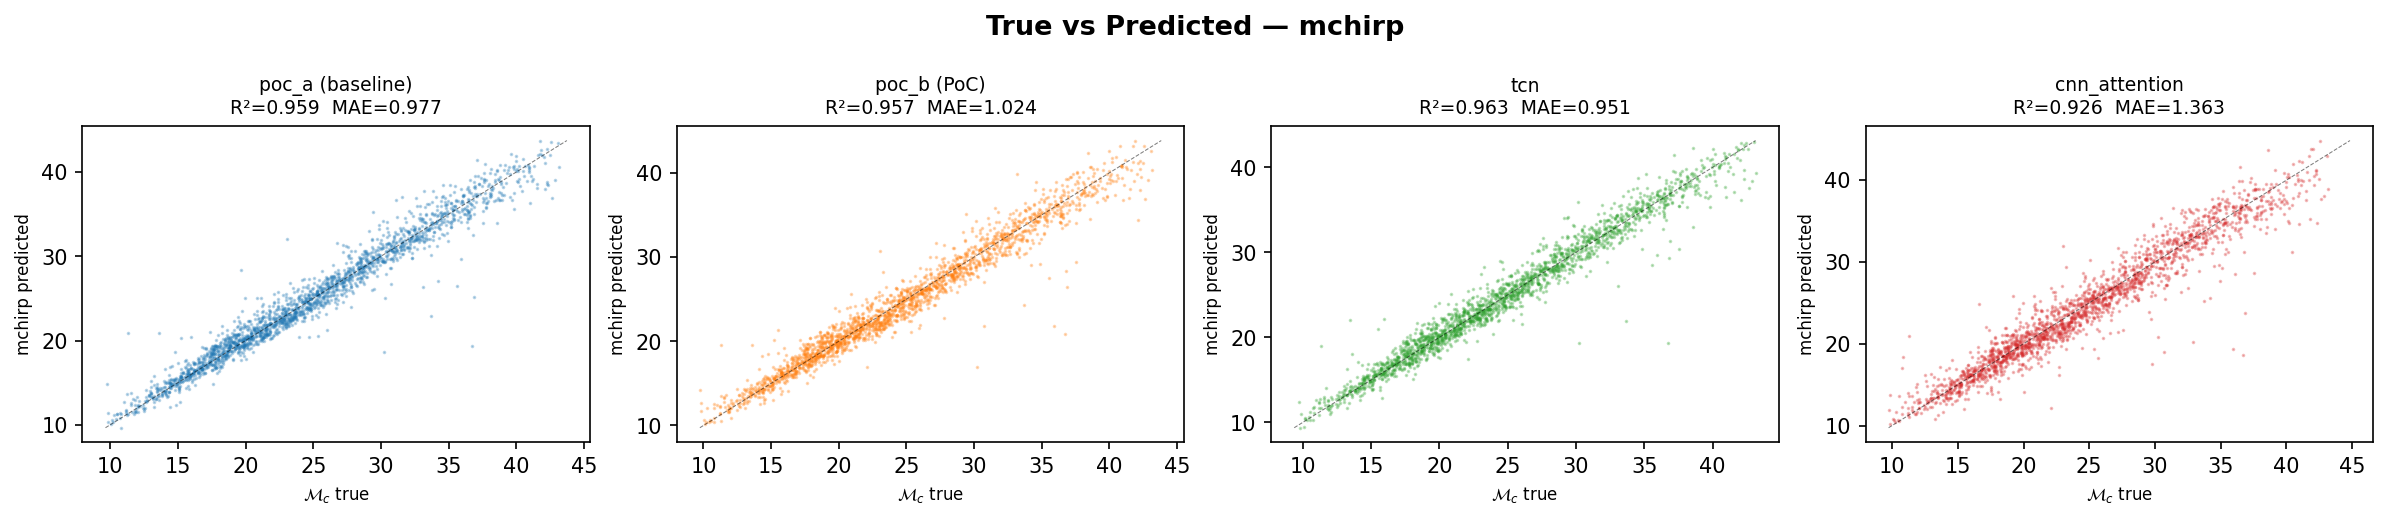
\includegraphics[width=\textwidth]{scatter_mchirp_20260720_234304.png}
    \caption[Chirp-mass recovery (positive control)]{Chirp-mass recovery on the validation set for the four Run~7 models ($R^2 = 0.93$--0.96).
    Together with merger time, SNR, and sky position, these positive controls establish that the shared trunk and training pipeline learn strain-derived parameters when the information is present.}
    \label{fig:phicpsi:mchirp}
\end{figure}